\documentclass[letterpaper]{article}

\usepackage[english]{babel}
\usepackage[utf8]{inputenc}
\usepackage{amsmath}
\usepackage[cm]{fullpage}
\usepackage{graphicx}
\usepackage{booktabs}
\usepackage{multicol}
\usepackage{pgfgantt}

\tikzset{every picture/.style={scale=0.72,transform shape}}

\newcommand{\MPB}{\textbf{MPB}\,}
\newcommand{\PERP}{\textbf{PERP}\,}



\title{Proxima Educational Robotics Platform Proposal}

\author{
Robert Nelson - 100845913 \\
Darren Stahl - 100858939\\
Hasith Vidanamadura - 100871538
}

\date{\today}

\begin{document}
\maketitle

\section{Introduction}

This is a proposal for the Proxima Educational Robotics Platform (\PERP). The \PERP is an ARM based robotics platform designed for teaching at Carleton. The project will run from September 2014 to March 2015. The group consists of Hasith Vidanamadura, Robert Nelson, and Darren Stahl, and will be supervised by Professor Pearce.

\section{Objective}

The objective of this project is to provide a consistent and modern hardware platform for use in courses throughout Carleton. This platform will be designed to provide a wide range of functionality, enabling multiple courses to base their lab work around it.

\section{Motivation}
Currently many of the courses taught by the SCE department use fairly out of date technologies; the Motorola 68000 and Intel 8086 both first appeared in the late 70s. While they are still useful for learning because of their simplicity, the technology and techniques they employ are significantly out of date, and there is a notable lack of focus on more modern embedded development.

Currently, there are two major processor architectures, x86 and ARM. Of these two architectures, ARM is gaining market share at a very significant rate, primarily in the embedded space. Not exposing students to embedded development with ARM puts them at a significant disadvantage in their careers, and this project aims to provide a pathway and a platform for teaching  modern embedded technologies. 

In addition to the modernization of the course content, the platform will also help recruitment by providing a very tangible and visible product that Carleton can take to school fairs, and demonstrate to prospective students. Finally, by keeping the cost of the board low, it will potentially allow students to purchase their own board, which they can then use throughout their entire program. This will give them extensive experience with a now prolific architecture, and teach them many modern embedded techniques that are largely neglected in the current course layout.
\section{Technical Overview}
The robotics platform will have two primary hardware components, the wireless monitor, and the main peripheral board. Users interact with the main peripheral board by plugging in a primary microcontroller board that contains an ARM-based microcontroller running user-written programs. The pluggable interface allows flexibility in the selection of the primary microcontroller board, and the end user is not constrained to a single interface or a vendor for their needs. This strategy also maximizes the usable lifetime of the platform, as a vendor rendering a specific development board obsolete will no longer affect the usability of the platform.


\subsection{Main Peripheral Board}
The main peripheral board (\MPB) will be a host for the primary microcontroller board and the wireless monitor. Additionally, peripherals on the \MPB could potentially include:

\begin{multicols}{2}
\begin{itemize}
\item Accelerometer
\item Gyroscope
\item Magnetometer
\item IrDA communication link
\item Temperature Sensor
\item Bump sensors
\item Microphone
\item Audio Codec
\item Digital to Analog Converter
\item Graphic LCD Screen
\item Keypad
\item Motor Controllers
\item SDCard
\item Real Time Clock
\item Line Detectors
\end{itemize}
\end{multicols}

\begin{figure}[!htp] \centering{
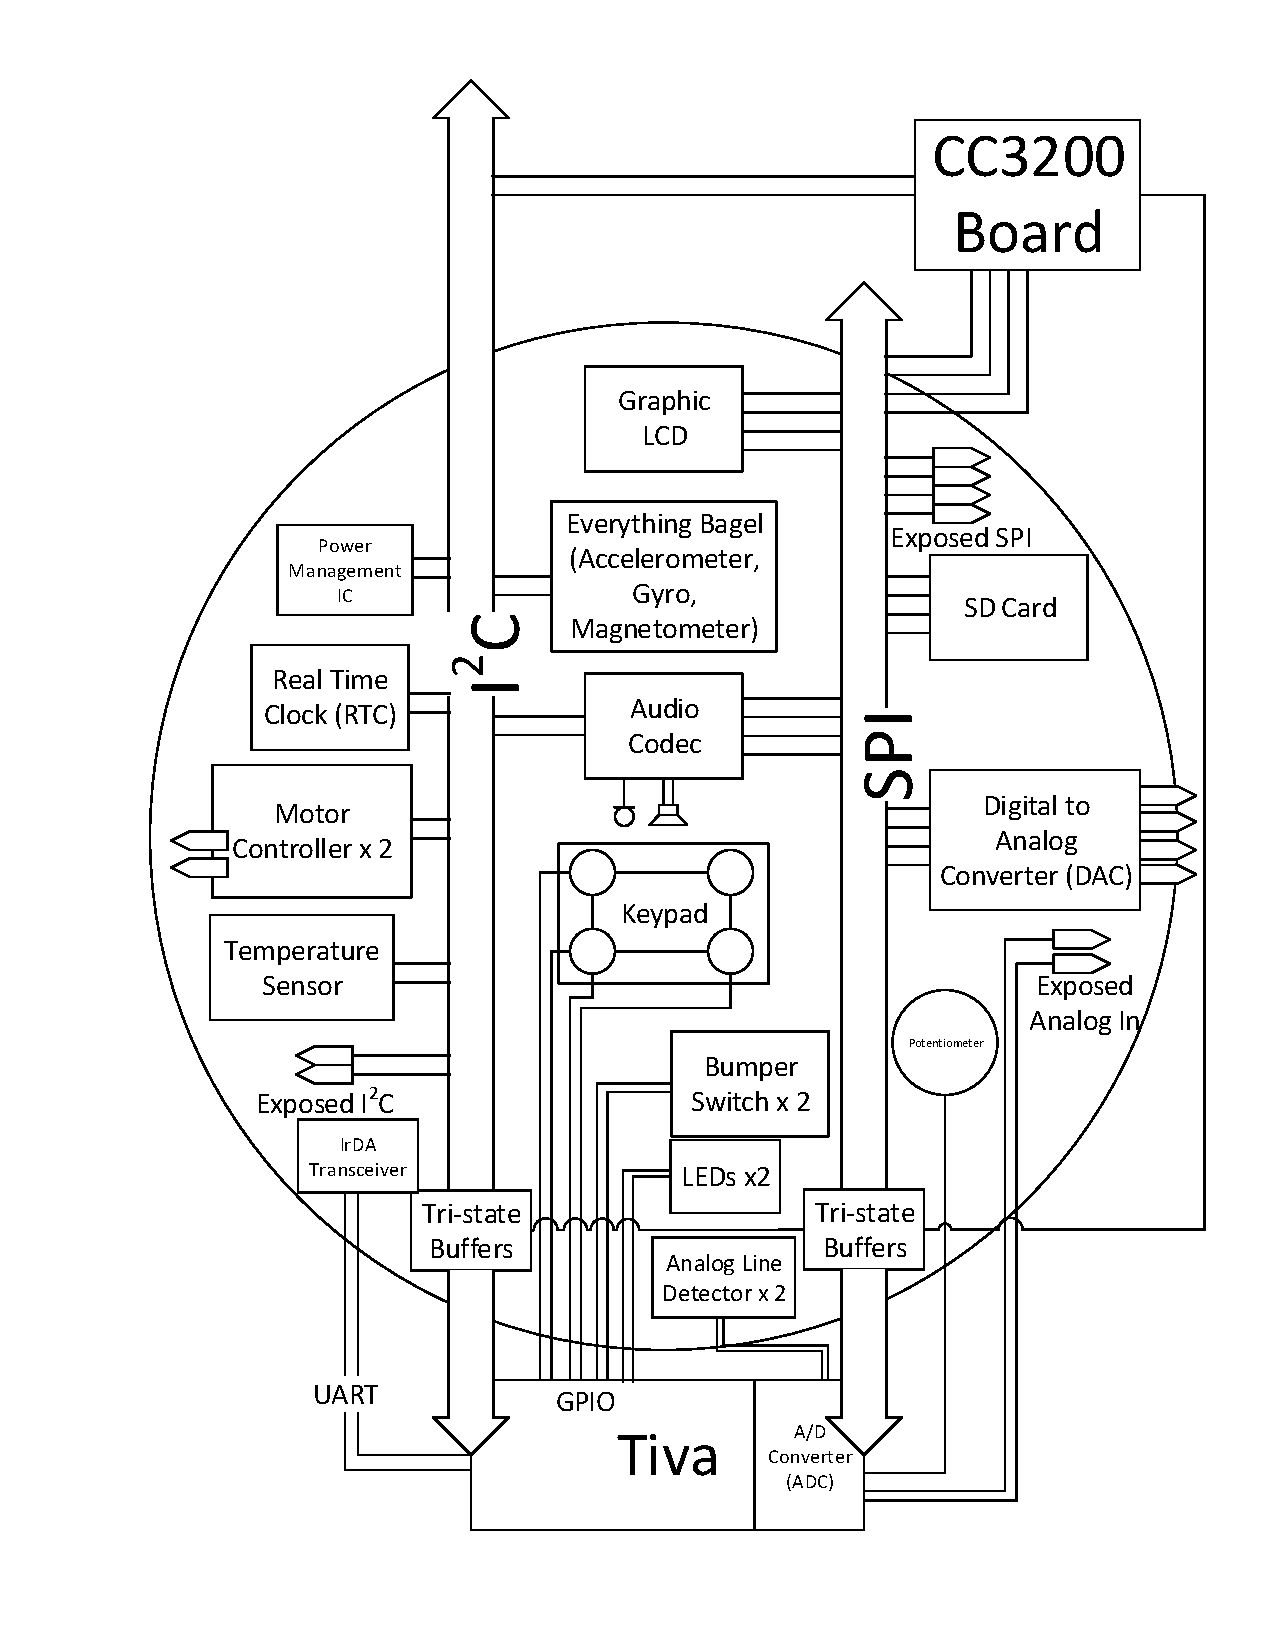
\includegraphics[scale=0.82]{block_diagram.pdf}}
\caption{Preliminary block diagram of the \PERP}
\label{fig:block_diagram}
\end{figure} 

These sensors will be chosen to maximize teachability, as these are common sensors the future engineer would interact with, as well as to maximize practicality, as these sensors provide useful data about the robotics platform's operating environment.

The sensors are connected using bus standards that are commonly used in modern embedded development contexts, and will provide students with experience and familiarity with said standards. Potential bus standards include SPI (Serial Peripheral Interface), I$^2$C (Inter-Integrated Circuit), parallel, and UART (universal asynchronous receiver/transmitter).

All electrical buses are also broken out onto easily accessible headers, so a user can add on functionality without modifying the \MPB.

A two-channel brushed-DC motor controller capable of driving a small pair of motors is provided on the \MPB for the user's convenience, and should suffice for the vast majority of the use cases. If the user wishes to control more motors, expansion interfaces will be provided.

The MPB handles power regulation and management for all the components in the system, and will be capable of providing current draw information and configurable battery monitoring.

To see a potential design of the peripheral board refer to Figure \ref{fig:block_diagram}.


\subsection{Wireless Monitor}
The wireless monitor is a self-contained module designed to sit on top of all the electrical buses that connect the \MPB to various sensors. Wireless connectivity is provided via IEEE 802.11b\/g\/n in a variety of modes.

\label{ss:operational-modes}
\subsubsection{Operational Modes}
There are two primary modes of functionality planned.

\begin{itemize}
\item{\textbf{Wireless Monitoring}}
The wireless monitor provides a browser accessible web portal through which the user can monitor sensors, control  each device, and interact with the platform directly without writing any code. This provides an easy verification of system status - the students can eliminate incorrect device functionality as a cause during debugging and can observe examples of incoming and outgoing data. 

The wireless monitor can electrically disconnect the primary microcontroller board from all the buses to eliminate the requirement for the student to perform bus arbitration with the wireless controller, and if required, can drive the entire platform without a primary microcontroller board connected.


\item {\textbf{Wireless Communication}}
The wireless monitor will also provide a communication channel for the end-user to interact with. Instead of forcing the end-user to understand the complexities of wireless connectivity, a user will be able to talk directly to the wireless monitor and have it act as a dumb pipe for transferring information to a host device (desktop computer or a smartphone connected to the wireless monitor) or to other instances of this robotics platform via a multicast system.  This opens up a range of possible communications methods and a variety of teaching outcomes.
\end{itemize}

\subsubsection{Design and Implementation}
The wireless monitor module will be designed and implemented as part of this project as a module-on-board, where the module is on a separate PCB, but soldered directly to the \MPB as a permanent component. The software stack enabling the functionality described in \ref{ss:operational-modes} will be a permanent part of the firmware and is not user accessible for modification easily to reduce the chance of an end user irrevocably rendering a key module unusable.



\section{Milestones}

The tentative project milestone sections are defined below. These milestones are in reference to Figure \ref{fig:gantt}, which describes the timing of the project.
\begin{table}[htp!]
\centering
\begin{tabular}{lcp{0.6\textwidth}}

\toprule
Group & Date Complete & Description\\
\midrule

Planning & Oct 6th & The planning phase involves understanding the problem and researching existing solutions. Requirements will be gathered from stakeholders, and input will be solicited on the project goals. This phase ends when all members have an understanding of the problem and what the planned solution is. During this phase professors teaching the courses aimed to be covered by the \PERP will be consulted to understand the expected learning outcomes. \\
HW Verification Suite & Nov 17th & The hardware verification suite will be a software suite that can exercise all of the peripherals in as many ways as possible (testing all usage is not feasible). This will be vital to the testing and verification of each hardware revision. The first version needs to be complete by the time the first hardware revision is ready for testing. \\
HW Rev 1 & Dec 1st & Hardware Revision 1 is about finalizing the components and basic board design, along with getting a production run to test. By the end of this phase the first revision board will have been designed, manufactured and tested with all bugs identified. The \MPB should have the basic functionality that we expect from the final product, but with some bugs and may require the addition of a few components. The CC3200 first revision board will also be complete at this milestone, but it is not expected to be fully operational by this milestone. \\
Bus Sniffers & Dec 8th & The bus sniffers will allow the WiFi monitoring station to collect all information that travels over the central buses. This functionality will be implemented and functional, but will not be graphically consumable. \\
Mon/Ctrl Website & Jan 5th & The monitoring and control web site will be implemented and usable. The website will be able to decode and display all of the signals that are collected by the Bus Sniffers. In addition, the website will allow commands to be sent to the peripherals. \\
HW Rev 2 & Jan 12th & This phase is the second revision of hardware designed and manufactured. It will consist of designing to fix any flaws that were found in the testing of the first revision boards, as well as adding any missing components to the board design. The end of this milestone is marked by a fully tested hardware revision, with most if not all bugs in the main board identified and solved, and minimal changes for revision 3. The CC3200 is still expected to be in flux. but should have a final form by the end of this milestone.\\
Peripheral Library & Feb 16th & The peripheral library will wrap all of the peripherals and provide a simple API for using them. \\
HW Rev 3 & Feb 23rd & Hardware Revision 3 is the final hardware revision. At the end of this phase, the final boards will both be feature complete and fully tested. There should be no bugs in the hardware design at this stage. This phase will end with at least 1 complete prototype assembled and ready for the final touches on the software development.\\
\bottomrule
\end{tabular}
\end{table}

\begin{figure}
\centering
\begin{ganttchart}{1}{29}
  \gantttitle{PERP}{29} \\
  \gantttitle[
    title label node/.append style={below left=-7pt and -6pt}
  ]{WEEKS:\quad1}{1}
  \gantttitlelist{2,...,29}{1} \\
  
  
  \ganttgroup{Planning}					{1}{4} \\
  \ganttbar{Research}					{1}{2} \\
  \ganttbar{Gather Requirements}		{1}{4} \\
  
  \ganttgroup{Hardware Rev1}			{4}{12} \\
  \ganttbar{Hardware Design Rev1}		{4}{6} \\
  \ganttbar{Manufacturer Lead Time}		{7}{10} \\
  \ganttbar{Testing Hardware Rev1}		{11}{12} \\
  
  
  \ganttgroup{Hardware Rev2}			{13}{18} \\
  \ganttbar{Hardware Design Rev2}		{13}{13} \\
  \ganttbar{Manufacturer Lead Time}		{14}{17} \\
  \ganttbar{Testing Hardware Rev2}		{18}{18} \\
  
  
  \ganttgroup{Hardware Rev3}			{19}{24} \\
  \ganttbar{Hardware Design Rev3}		{19}{19} \\
  \ganttbar{Manufacturer Lead Time}		{20}{23} \\
  \ganttbar{Testing Hardware Rev3}		{24}{24} \\
  
  
  \ganttgroup{Department Objectives}	{1}{29} \\
  \ganttmilestone{Proposal Draft}		{2} \\
  \ganttmilestone{Progress Report}		{14} \\
  \ganttmilestone{Oral Presentation}	{19} \\
  \ganttmilestone{Final Report Draft}	{27} \\
  \ganttmilestone{Poster Fair}			{29} \\
  
  
  \ganttgroup{Software Development}		{1}{26}  \\
  \ganttbar{Setup Dev Environment}		{1}{4}   \\
  \ganttbar{Hardware Verification Suite}{5}{10}  \\
  \ganttbar{Peripheral Library}			{5}{23}  \\
  \ganttbar{Bus Sniffers}				{11}{13} \\
  \ganttbar{Monitoring/Control Website}	{14}{17} \\
  \ganttbar{Implement Lab Exercises}	{18}{26} \\
\end{ganttchart}
\caption{Timeline of milestones and predicted schedule}
\label{fig:gantt}
\end{figure}

\pagebreak
\section{Benefits}
This project has the potential to have a positive impact on the school, the professors and the students, each in a unique way. The sections below will discuss how this project will positively impact each group.

\subsection{School}
The construction of a robotics teaching platform designed and built by Carleton students will be a very useful recruiting tool for the CSE and DOE departments. The robot will be portable enough to take to recruiting events, allowing potential students to see the possibilities that are available to them if they enroll. Several key features of the platform, such as the wireless controllability, also allow for some appealing demonstration possibilities to capture the interest of potential high school students.

\subsection{Professors}
If there is one consistent platform that many different courses will use, professors will be able to share notes and code amongst themselves reducing the preparation burden on any one person. In addition, having one platform service multiple courses will allow for more realistic labs to be designed, because the students will already be familiar with the environment, eliminating the need to re-teach how to accomplish basic tasks on it. 
\subsection{Students}
ARM is a very prominent player in the embedded market currently, so learning to develop on an ARM platform is very beneficial when job hunting. In addition, the low cost of the Proxima Platform will allow students to purchase the equipment once and use it for several courses, reducing their term over term costs. It will also, once purchased, be an environment that will be familiar and flexible enough to be used in projects in third and fourth year.
\section{Budget}
This project will require building several revisions of a hardware platform, and as such will require funding to purchase the components and have the PCB manufactured. Several revisions are planned for to ensure that a quality product is developed and that any mistakes made in early revisions are fixed before the final project is complete.
\subsection{Prototyping Cost Estimates}
The cost estimates below are for each revision, and are rough approximations of costs, because board sizes and components have not been chosen.
\begin{multicols}{2}
\begin{itemize}
	\item Peripherals (Sensors, LEDs, etc.) - \$30.00
    \item WiFi processor - \$20.00
    \item LCD Module - \$10.00
    \item Supporting Passive Components - \$10.00
    \item 2 Motors - \$5.00
    \item Keypad - \$5.00
    \item Main PCB - \$30.00
    \item WiFi PCB - \$20.00
    \item Power supply - \$5.00
    \item Battery - \$10.00
\end{itemize}
\end{multicols}

This comes to a total of approximately \$115.00 for each revision if no mistakes are made. To account for the reality that mistakes will be made, this cost will be doubled during the prototyping phase to ensure that if a problem arises or a mistake is made during the assembly of a revision's prototype, that a backup can be made. The current plan for assembly calls for three main revisions, and one backup revision, bringing the total cost up to approximately \$950.00. In addition to the actual prototypes, in order to allow for the software suite to be developed in parallel, some pre-built dev boards will be purchased. The approximate cost of each of these dev boards is \$25.00 and two different boards will be required for each team member (one for main processor, one for WiFi processor.) This additional cost brings the total budget up to \$1100.

\subsection{Volume Production}
The costs outlined in the previous section are only valid during the prototyping phase. Once the design is stable the vast majority of the components in this design will benefit from significant price reductions when purchased in bulk. As such, the cost per unit (at a hundred estimated units) will decrease by an estimated 30\% reducing the cost of each \MPB below \$100.00. Further demand will reduce the pricing further, as more units are available to absorb the fixed costs.

\end{document}